\documentclass[10pt]{beamer}

\usetheme[compress]{Berlin}
\usepackage[utf8]{inputenc}
% Alternative Optionen
\setbeamertemplate{navigation symbols}{}
%\usepackage{beamerthemeshadow}
%\beamersetuncovermixins{\opaqueness<1>{25}}{\opaqueness<2->{15}}


%\usepackage{beamerthemesplit}

\usepackage{graphicx}

%\setbeamerfont{parent A}{size=\large}
%\setbeamerfont{parent B}{series=\bfseries}
%\setbeamerfont{child}{parent={parent A, parent B},size=\small}
\setbeamerfont{small}{size=\small}


%============================================================================

\title{Concept - SBM-System / ElementSpace }
\author{Andreas Hauck}
\date{\today}

\begin{document}

% =================================
\begin{frame}
 \titlepage 
\end{frame}

% =================================

\begin{frame}
\frametitle{Outline}
\tableofcontents
\end{frame}

% =================================

\section{Drawbacks of Current Concepts}
\begin{frame}[fragile]{AlgebraicSystem / OLAS}
  \begin{itemize}
  \item System matrices only adressable as whole block via \verb+pdeId+, no further distionction in different solution types within one PDE possible
  %\begin{itemize}
  %\item No block solver possible
%\item No Schur-Complement method 
%  \end{itemize}
  \item OLAS does not know about the nature of the problem
  \item Status information of OLAS just written in plain files
  \end{itemize}
\end{frame}

% =================================

\begin{frame}[fragile]{Equation Handling}
\begin{itemize}
 \item Cumbersome numbering with similar loops for nodes/edges/faces/elements
 ( global $\rightarrow$ pdeLocal $\rightarrow$ eqn)
\item No discontinuous mapping possible
\item EqnMap can not know how to handle higher order modes (boundary conditions etc.)
\begin{itemize}
\item Set modes to zero?
\item Map boundary function to coefficients?
\end{itemize}
\end{itemize}
\end{frame}

% =================================

\begin{frame}[fragile]{Elements / Ansatz Functions}
\begin{itemize}
 \item Currently choice of shape functions encoded in {\tt AnsatzFct}-class
\item Nested \verb+if+-statements in each Element subclass for Lagrange/Legendre/Spectral
\item Shape Mapping (Jacobian Determinant, local $\leftrightarrow$ global coordinates) not independent of FE-approximation (only iso-parametric concept)
\item Axial symmetry explicit encoded in bilinear forms
\item No flexible choice of integration order possible (order for stiffness matrix lower than for mass matrix)
\end{itemize}
\end{frame}

% =================================

\begin{frame}[fragile]{(Bi-)Linearforms}
 \begin{itemize}
  \item Class structure of many forms too complicated (e.g. MechStressStrain $\leftrightarrow$ LinElastInt)
\item Calculation of Jacobian Matrix too often (BDB-Form, B-Operatoer etc.)
\item Inconsistent feature support of bilinearforms for 
\begin{itemize}
\item rotation of material data / arbitrary coordinate systems
\item material tensor instead of isotropic behavior
\item usage of math parser
\end{itemize}
 \end{itemize}
\end{frame}

% =================================

\begin{frame}[fragile]{Relicts of Nodal Stone Age}
  \begin{itemize}
\item Boundary conditions only mapped to nodal degrees of freedom
\item Iterative coupling works just on nodes / element interior
\item HDF5-Writer currently just handles nodal / element dofs
\end{itemize}
\end{frame}

% =================================

\section{New Concepts}
\begin{frame}[fragile]{Overview of new Concepts}
\begin{itemize}
 \item New Element hierarchy
\item FESpace 
\item SBM-System
\item Equation Numbering System
\item Shape Mapping Concept
\end{itemize}
\end{frame}


\subsection{New Element Hierarchy}
\begin{frame}[fragile]{Element classes}
\begin{itemize}
 \item Distionction of elements w.r.t. function space they are belonging (H1 / HCurl / HDiv / L2) 
\end{itemize}
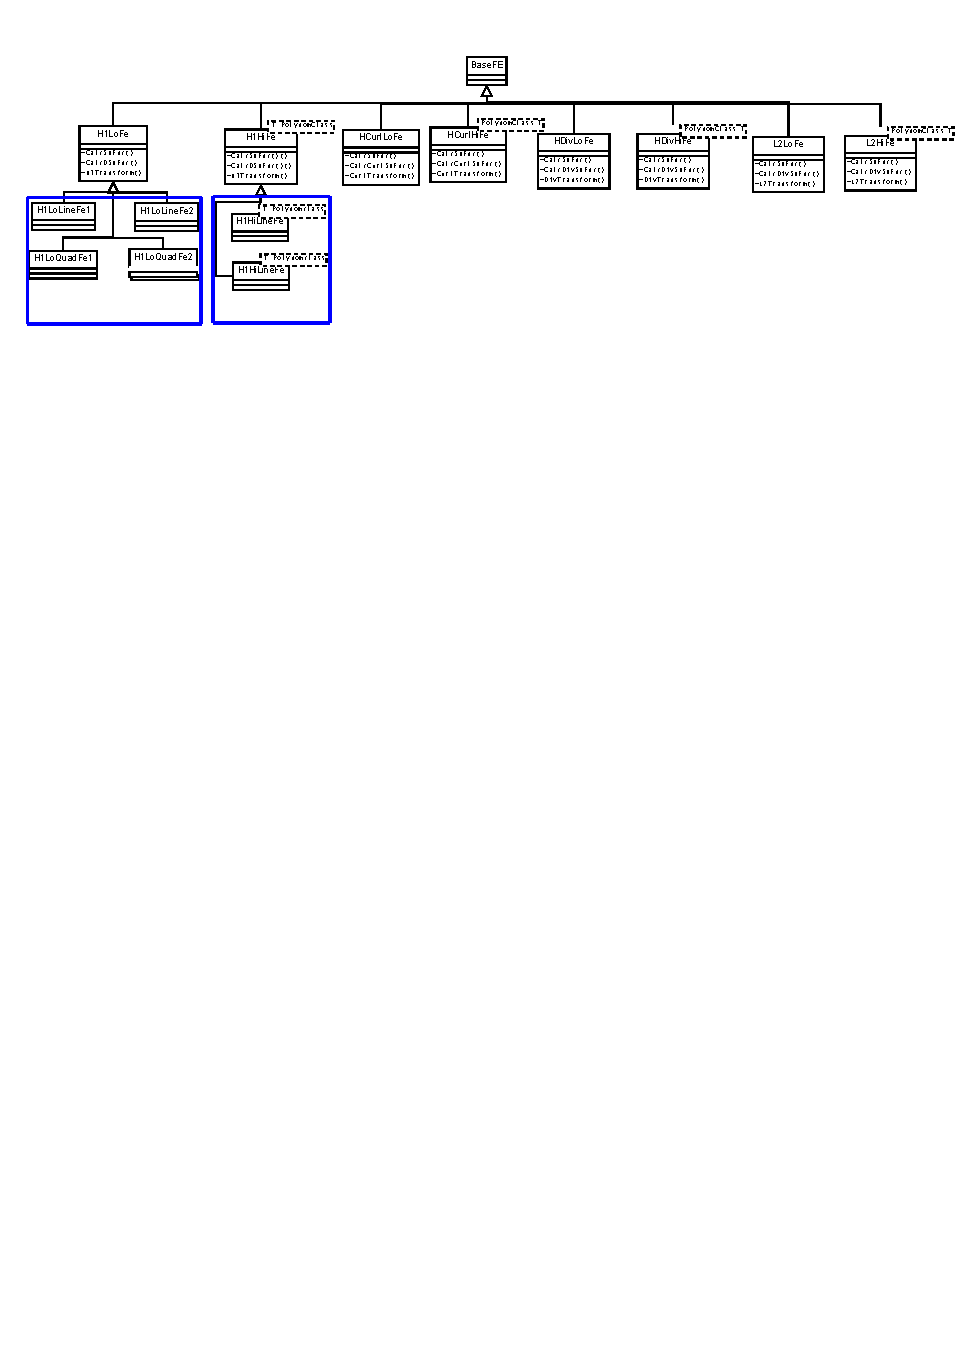
\includegraphics[width=12cm]{elems.pdf}
\end{frame}

\begin{frame}[fragile]{Element classes (cont'd.)}
\begin{itemize}
\item Distinction of lower order (Lagrange-type) and higher order space (arbitrary order) 
\item As the shape for all e.g. quadrilaterals is the same, we keep the geometric information of the element (nodes, edges, faces, dimension) in a common structure {\tt RefElemShapes}, in where we can access the geometric information using the {\tt FeType}
\begin{verbatim}
   // get corner coordinates for QUAD4
   Matrix<Double> & cornerCoords = 
        RefElemShapes::shape(QUAD4).cornerCoords;
\end{verbatim}
\item Higher order elements can use different polynomials (Jacobi, Legendre, etc.)
\end{itemize}
\end{frame}

\subsection{FeSpace}
\begin{frame}[fragile]{FeSpace}
\begin{itemize} 
\item Collects pointers to H1 / HCurl / HDiv FE-elements (class \verb#Elem# gets rid \verb#BaseFE# pointer), so it acts as {\color{red} Common interface for all reference FE elements of one given type (H1Lo/Hi, HCurlLo/Hi ...)}
\item Returns FE-Element for geometric element
\item Performs equation numbering (replaces EqnMap-class)
\item Has general methods to change attributes of ALL its elements, e.g.
\begin{itemize}
\item Order of shape functions
\item Integration order
\item Which polynomials to use for higher order elements (Legendre, Jacobi)
\end{itemize}
\end{itemize}
\end{frame}

\begin{frame}[fragile]{Equation Numbering}
Perform Re-numbering transparantly in OLAS 
\begin{itemize}
  \item Allow for discontinuous mapping of equation numbers
  \item FeSpace registers at OLAS and obtaines FunctionId (formerly the pdeID)
  \item Each solution in the FeSpace has equation numbers starting from $1,\dots,n$
  \item FeSpace can optionally decide to create alternative two level grouping of equations (majorBlockId, blockId), which map to physical matrix blocks in the SBMSystem (see section about SBM-system)
 \end{itemize}
\end{frame}


\begin{frame}{Equation Numbering (cont'd.)}
The FeSpace should allow for a unified mapping of nodes/edges/faces/interior to equation numbers, for the continuous, as well as for the discontinuous case.
\begin{block}{Mapping Scheme}
\usebeamerfont{small}
\begin{tabular}{c|c|c}
& continuous & discontinuous \\ \hline
(elemNr,nodeNr) & map$<$nodeNr, EqnNr$>$ & map$<$(elemNr,nodeNr),eqnNr$>$ \\
(elemNr,edgeNr) & map$<$edgeNr, EqnNr$>$ & map$<$(edgeNr,nodeNr),eqnNr$>$ \\
(elemNr,faceNr) & map$<$faceNr, EqnNr$>$ & map$<$(faceNr,nodeNr),eqnNr$>$ \\
\end{tabular}
\end{block}
\end{frame}
\subsection{FeFunction}
\begin{frame}{FeFunction}
 The FeFunction generalizes the NodeStoreSolution class. 
\begin{block}{It ...}
\begin{itemize}
 \item stores the coefficients of a solution
\item knows about its boundary conditions (hold the BCs objects) and can map them to its coefficients (projection based interpolation)
\item can map itself to another function or to a Node/Elem-Result object (for postprocessing)
\item knows about its FeSpace (which knows the equations numbers) as well as its FunctionId (for OLAS)
\end{itemize}

\end{block}


\end{frame}


\subsection{SBM-System}
\begin{frame}[fragile]{Super Block Matrix (SBM) System}
 \begin{block}{Original idea by Marcus Mohr}
\begin{itemize}
 \item Matrix-/ Vector entries are themself matrices
\item Address block(s) via pdeID
\end{itemize} 
\end{block}

\begin{block}{More flexible way of addressing blocks, e.g.}
\begin{itemize}
  \item SolutionType (several solutions within on PDE, e.g. mixed formulations)
\item Node / Edge / Face / Inner dofs
\item Higher Order $\leftrightarrow$ Lower Order Functions
\item Dual / Primal Ansatz space (Simons NC-interfaces)
\item Spatial separation / different regions (Local Timestepping)
 \end{itemize}
\end{block}
\end{frame}

% =================================
\subsection{Equation Numbering / Block Adressing}
\label{sec:blockadress}
\begin{frame}[fragile]{SBM-System (cont'd.)}
Allow for more flexible solution strategies 
\begin{itemize}
  \item Omit sub-blocks (e.g. static condenstation)
  \item Schur-complement method
  \item Block-Jacobi solver
 \end{itemize}
\end{frame}

% =================================

\begin{frame}[fragile]{SBM-System (cont'd.)}
Up to now, OLAS just knows pdeIDs and equation numbers.
The new concept allows three views onto the system.
\begin{block}{Access strategies}
 \begin{itemize}
 \item {\color{red}(matrixId, row/col)} SBM-internal view on entries
  \item {\color{red}(functionId, eqnNr)} solution-oriented view from CFS++
  \item {\color{red}((mBlockId, blockId), row/col)} Alternative Logical view from CFS++ (e.g. local time stepping)
 \end{itemize}
\end{block}
 OLAS internally performs the mappings 
\begin{itemize}
 \item{\color{red}(functionId, eqnNr) $\rightarrow$ (matrixId, row/col)}
\item {\color{red}((mBlockId, blockId), row/col) $\rightarrow$ (matrixId, row/col)}
\end{itemize}
\end{frame}

\begin{frame}[fragile]{Example}
We consider a mixed PDE with pressure $p$ and velocity $v$ as dofs, additionally split up in two regions $1$ and $2$ (superscript). The resulting systems looks like (only diagonal and upper diagonal entries shown)
\begin{center}
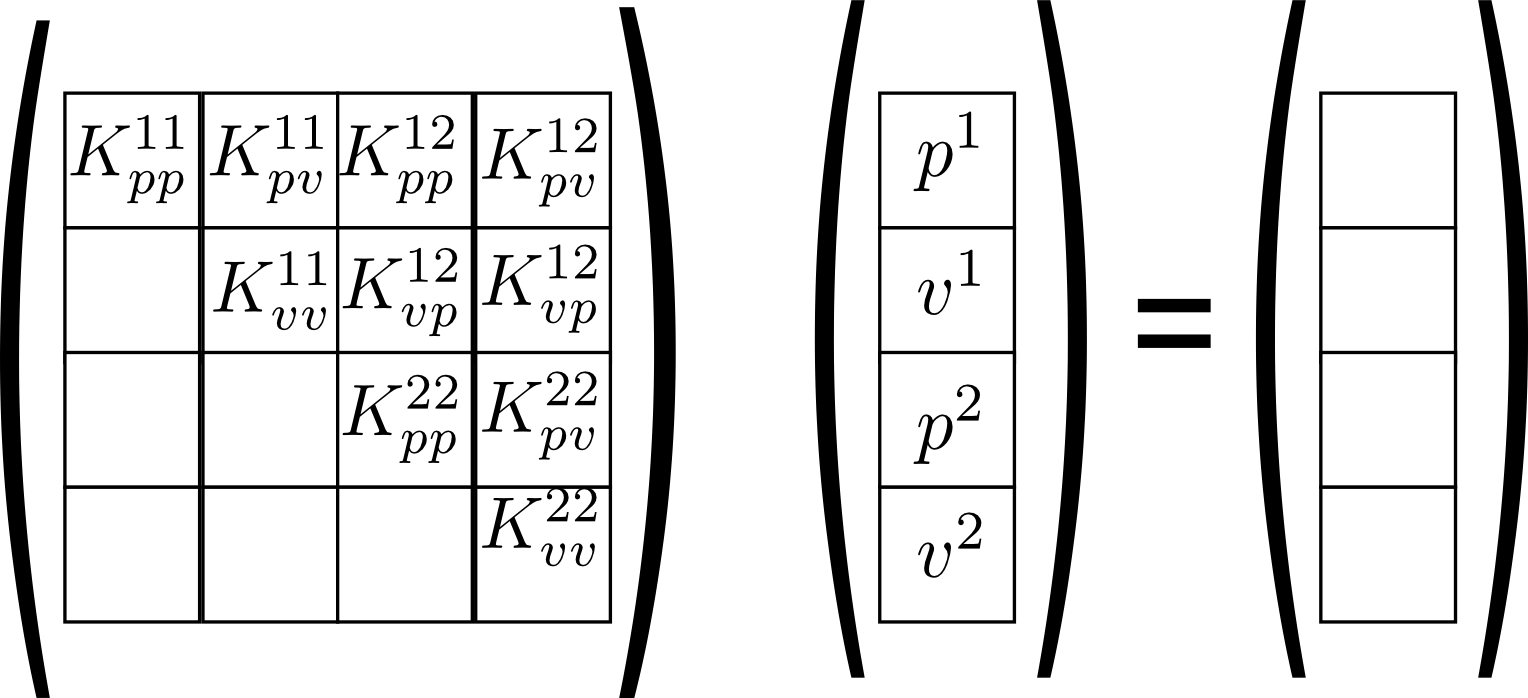
\includegraphics[width=6cm]{system1.png}
\end{center}
\end{frame}

\begin{frame}[fragile]{Example - Physical View}
The SBM system has a consecutive numbering of the rows/columns containing the matrices, e.g. the matrix $K_{pp}^{12}$ has the \emph{coordinate} (1,2).
\begin{center}
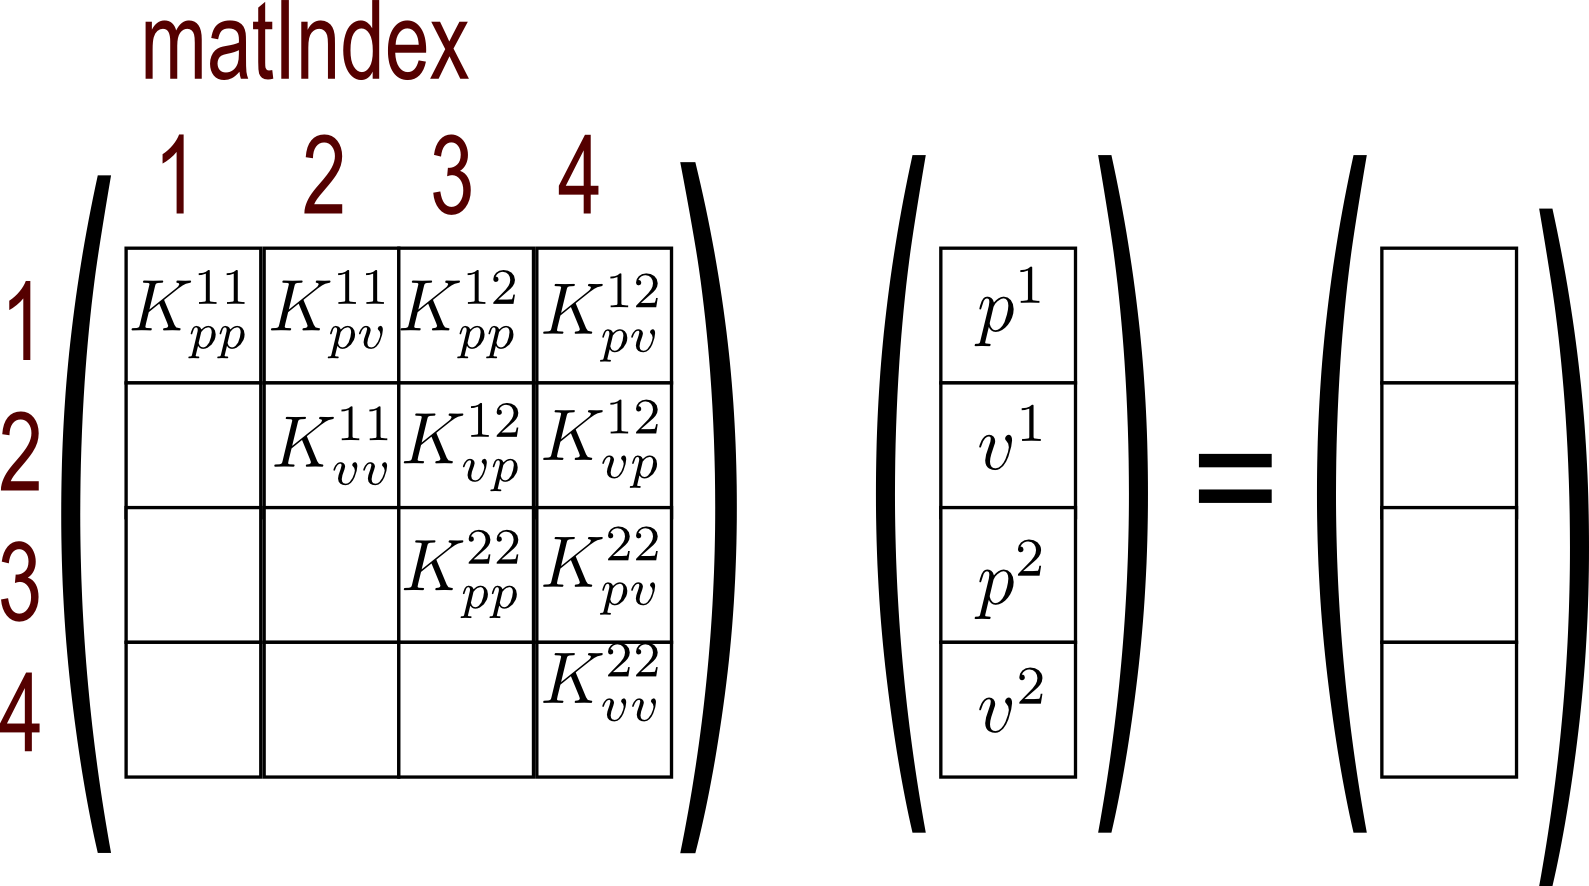
\includegraphics[width=6cm]{system2.png}
\end{center}
This is the OLAS internal view. Outside OLAS, no one needs to know the \emph{exact} row / column index of the matrices!
\end{frame}

\begin{frame}[fragile]{Example - Solution oriented view}
 CFS normally adresses the entries in a combination of {\color{red} (functionId, eqnNr)}, which OLAS maps to a matIndex and a row / column.
\begin{center}
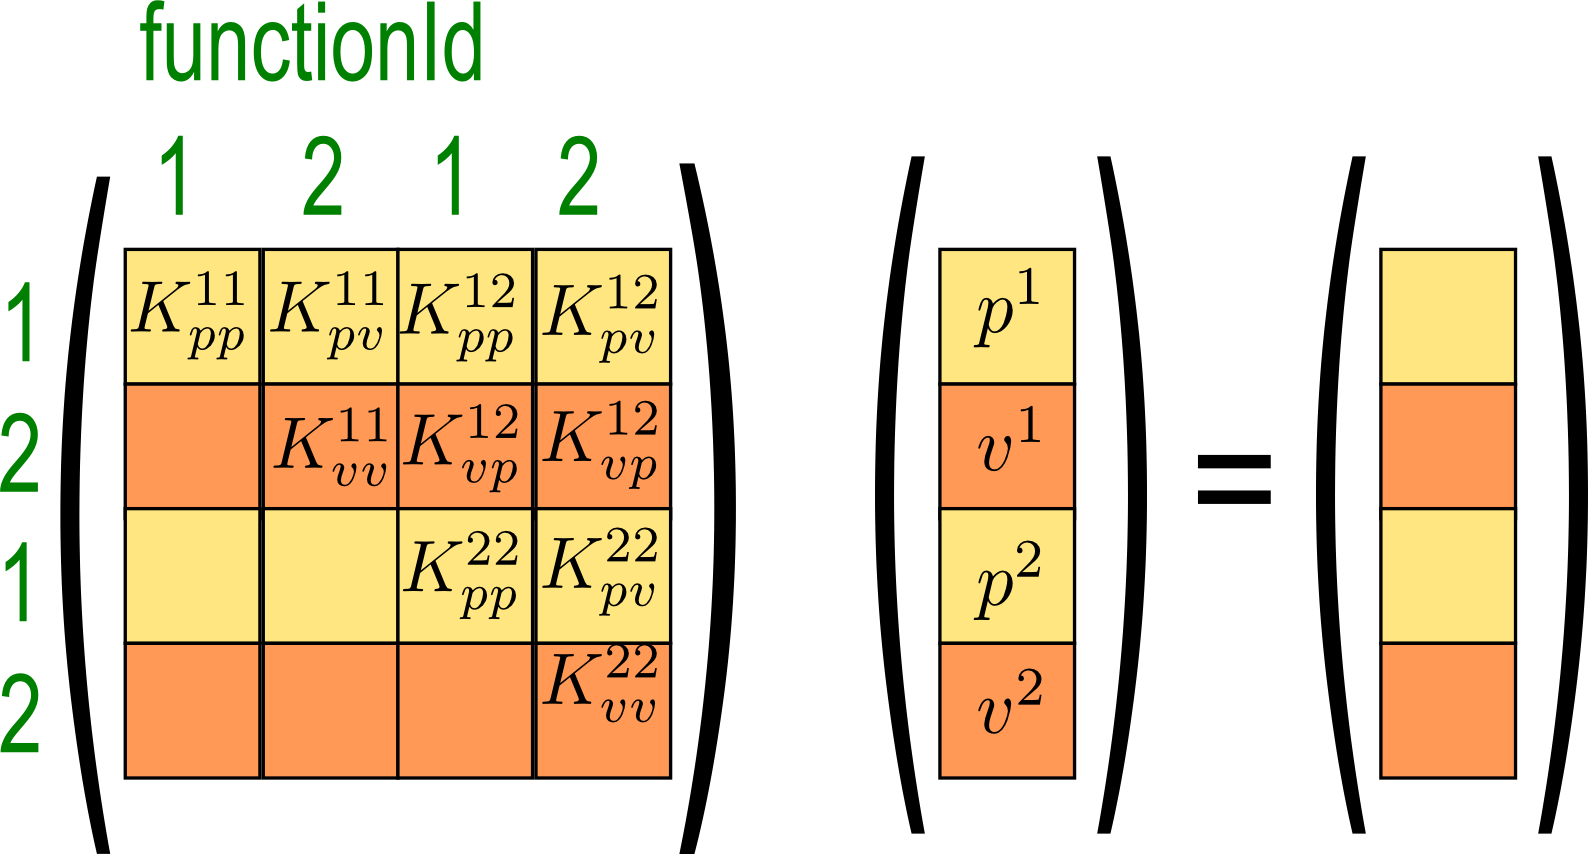
\includegraphics[width=6cm]{system3.png}
\end{center}
This should be the normal view from CFS++, e.g. during matrix / vector assembly and when accessing the solution. If the user requests the solution for $p$, OLAS has to collect the entries from the blocks $p^1$ and $p^2$ and copy them into a SingleVector.
\end{frame}

\begin{frame}[fragile]{Example - Alternative Logcial View}
 Two level grouping  ({\color{blue}mBlockId},{\color{magenta}blockId}) (as requested by the FeSpace):
\begin{itemize}
\item Major Block level (mBlockId): Address all unknowns in Region 1 and 2
\item Block level (blockId): Address different solution unknowns within on region
\end{itemize}
\begin{center}
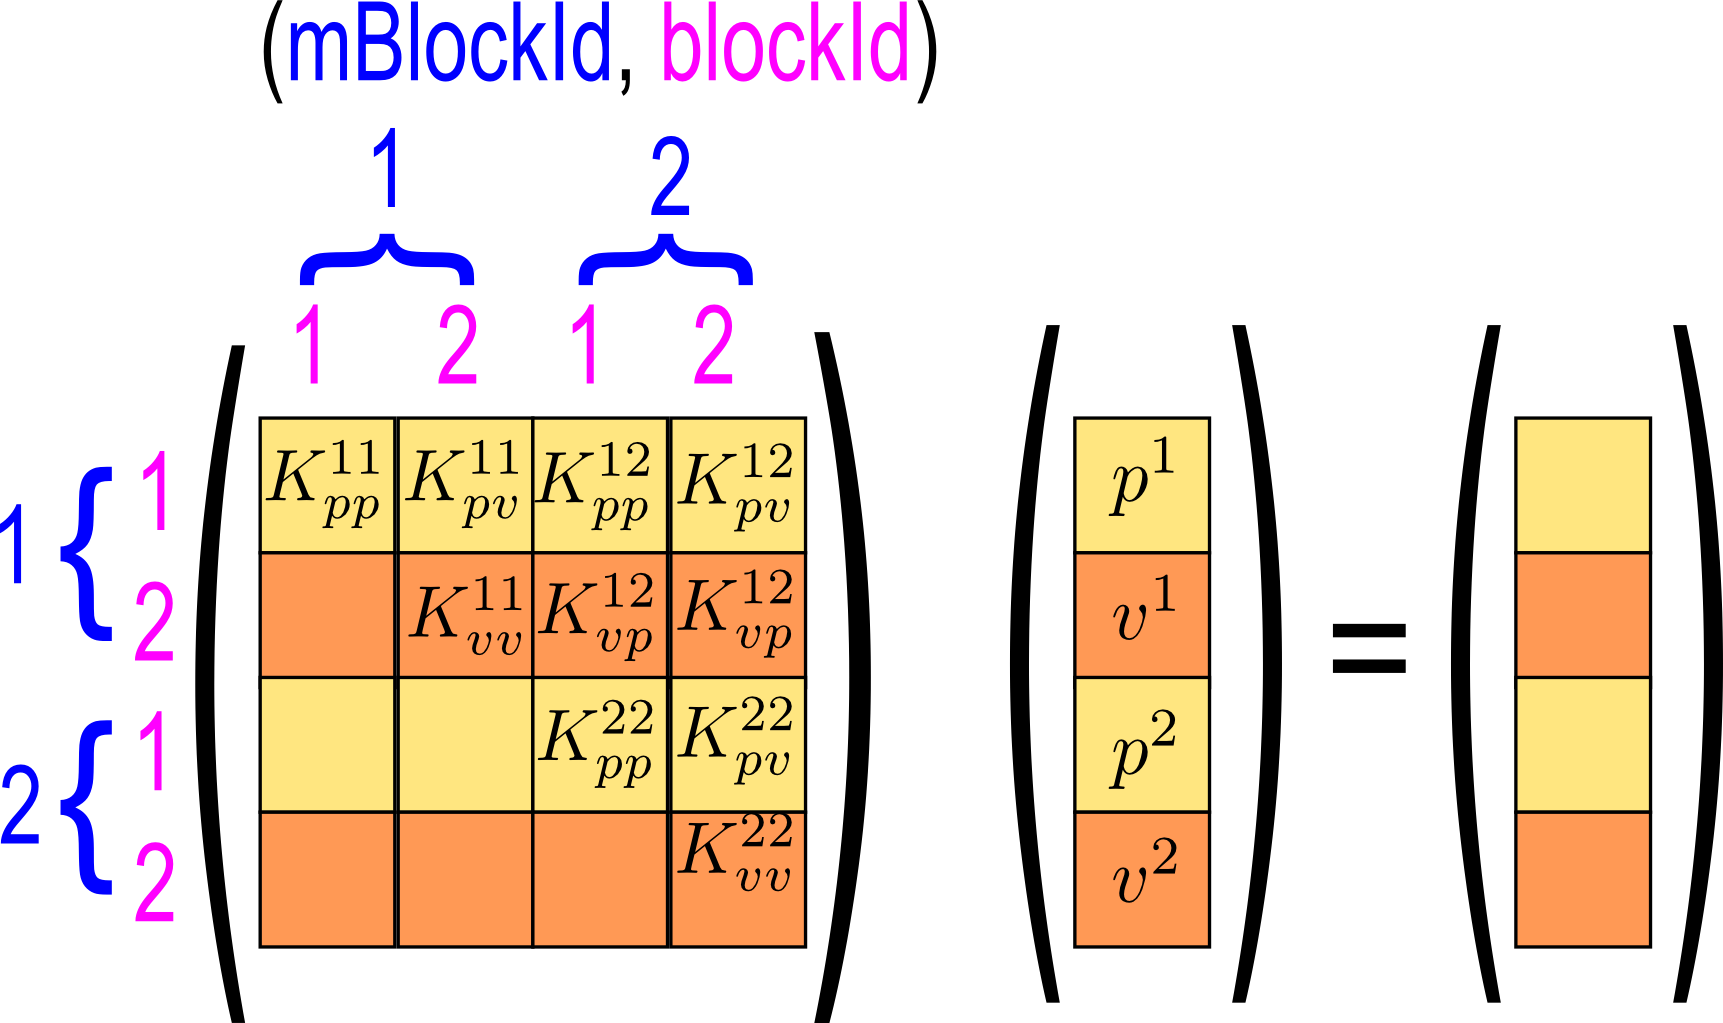
\includegraphics[width=5cm]{system4.png}
\end{center}
This can be used for local time stepping, e.g. request block for region 1 (Sub-SBM vector) and solve locally. Using the blockId, we can access $p^1$ and $v^1$ within one major block.

\end{frame}

% =================================




\subsection{Shape Mapping}
\begin{frame}{New Shape Mapping concept}
 to be written ...
\end{frame}

\subsection{More Reusability}
\begin{frame}{Modify BilinearForms structure}
 to be written ...
\end{frame}

\section{Who's Doing What / Timetable}
\begin{frame}{Workplanning - Simon}
 \begin{itemize}
  \item Concentrate on OLAS
\item Implement block mapping concept
\item Implement simple Schur complement solver
 \end{itemize}
\end{frame}

\begin{frame}{Workplanning - Andi Hauck / Andi Hüppe}
\begin{enumerate}
  \item Comment out all PDEs and Forms except the simple elecPDE and the linElecInt integrator to get a \emph{lightweitht} implementation playground
  \item Create FeSpace base class and FeSpaceH1Lo, which collects all the pointers to the Lagrangian elements
\item .... (to be discussed on the phone)
 \end{enumerate}
\end{frame}



\section{Open Questions}
\begin{frame}{Open Questions}
 ???
\end{frame}


\end{document}
